\documentclass[12pt]{article}

\usepackage{Code/Fonctions}

\usepackage[utf8]{inputenc}
\usepackage{graphicx}
\usepackage{wrapfig}
\usepackage{url}
\usepackage{hyperref}
\usepackage{subcaption}
\usepackage{array}
\usepackage{caption}
\usepackage{geometry}
\geometry{margin=2.5cm}
\usepackage[francais]{babel}
\usepackage[T1]{fontenc}
\usepackage{enumitem}

\author{Killian Mathias}{I}
\author{Matthéo Girardclos}{II}
\title{Génération procédurale de décors}
\reportType{Projet de recherche documentaire}
\academicInfo{Département Informatique UFR-ST}{Université Marie et Louis Pasteur}{2024 - 2025}
\titleImage{assets/background_1}
\date{\today}

\begin{document}

\maketitle
\newpage

\tableofcontents
\newpage

\section{Introduction}

En informatique, la génération procédurale fait référence à la création automatique de contenu numérique, que ce soit des éléments en 2D ou 3D, des scénarios, des dialogues, ou même des niveaux de jeu. Cette technique s'appuie sur des algorithmes qui permettent de produire une grande quantité de contenu sans nécessiter l'intervention directe d'un humain. Elle est particulièrement prisée dans les secteurs du jeu vidéo et du cinéma, où elle aide à créer des environnements variés et immersifs.  Un exemple marquant de cette méthode est le jeu Minecraft, qui génère un monde ouvert de manière procédurale grâce à différentes couches d'algorithmes. D'autres jeux, comme Terraria ou No Man’s Sky, utilisent également cette approche pour offrir des mondes dynamiques et uniques.\par
Créer des décors qui soient à la fois aléatoires et cohérents représente un vrai défi. Par exemple, modéliser des reliefs comme des montagnes ou des plaines peut être assez complexe. La génération procédurale aide à surmonter ce problème en appliquant des algorithmes adaptés, ce qui évite de devoir concevoir chaque carte de jeu à la main.\par
Dans le cadre de ce projet, notre but est de développer une version simplifiée de Terraria, un jeu de survie en 2D. Ce jeu, jouable en solo ou en multijoueur, permet aux joueurs d'explorer un monde divisé en biomes, de récolter des ressources et d'interagir avec leur environnement. Nous allons nous concentrer sur la génération du monde, des biomes et éventuellement des grottes, tout en veillant à optimiser l'implémentation pour garantir de bonnes performances.
\begin{figure}[!h]
  \centering
  \begin{subfigure}[b]{0.4\textwidth}
    \centering
    
\includegraphics[width=0.5\textwidth]{assets/nomanssky.png}
    \caption{No Man's Sky}
  \end{subfigure}
  \hspace{0.6cm}
  \begin{subfigure}[b]{0.4\textwidth}
    \centering
    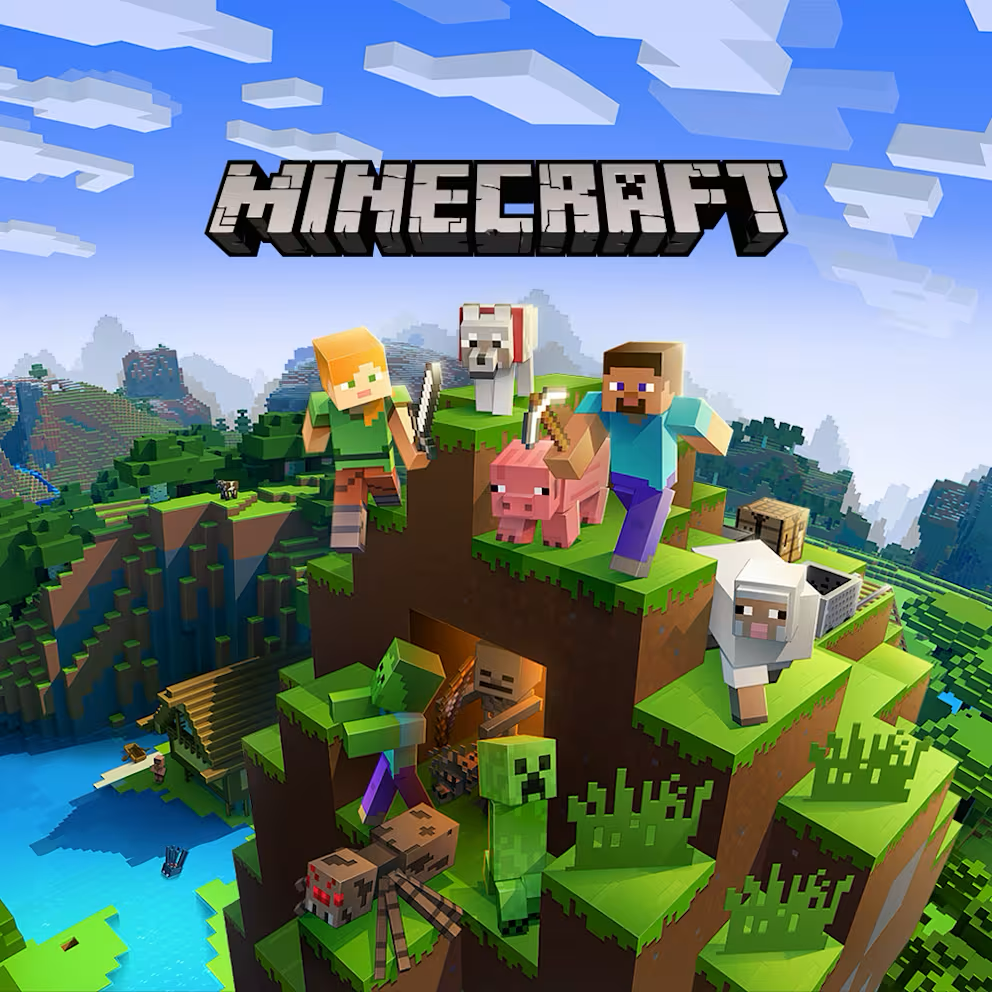
\includegraphics[width=0.5\textwidth]{assets/minecraft.png}
    \caption{Minecraft}
  \end{subfigure}
  \hspace{0.6cm}
  \label{games}
  \caption{Jeux utilisant la génération procédurale}
\end{figure}

\section{Différentes approches}

Afin de générer procéduralement un décor il existe plusieurs approches. Tout d'abord, les objectifs d'une implémentation à une autre ne sont pas exactement les mêmes, cependant cela reste de la génération procédurale. Dans cette section, nous présenterons plusieurs méthodes populaires, en les analysant sous l’angle de leur efficacité et de leur applicabilité à notre projet de génération d’un monde 2D de type Terraria.\par
Tout d'abord afin de répondre à nos besoins nous devons créer des paysages avec des reliefs réalistes.
\newpage
\vspace{1cm}
\subsection{Génération de terrains et de reliefs}

\begin{wrapfigure}{r}{0.2\textwidth} % 'r' pour droite, largeur ajustée
  \centering
  
\includegraphics[width=0.18\textwidth]{assets/Perlin_noise.jpg}
  \caption{Bruit de Perlin à 2 dimensions}
  \label{perlin}
\end{wrapfigure}

Pour créer des paysages avec des reliefs il existe deux algorithmes qui sont respectivement le bruit de Perlin et le bruit Simplex.\par
D'après la page Wikipédia \cite{perlin}, le bruit de Perlin, développé par Ken Perlin en 1985, est un système de génération pseudo-aléatoire. Ce dernier cherchait à éliminer le look "machinique" des effets spéciaux du film \textit{TRON.} Son utilité principale est la génération procédurale de décors au nombre de dimensions que l'on souhaite mais il est plus fréquemment utilisé à 2 ou 3 dimensions. Nous rentrerons dans les détails de cet algorithme plus tard.\par
Le bruit Simplex \cite{simplex_noise} a également été créé par Ken Perlin en 2001 avec le but de remédier aux limites de son algorithme précédent. Il est assez similaire au bruit de Perlin, mais il est plus efficace et est généralement utilisé pour travailler avec des espaces à plus de 3 dimensions. Nous ne verrons pas en détail cet algorithme, car bien qu'il soit plus performant, il est moins documenté que son prédécesseur et donc logiquement plus difficile à comprendre.
\vspace{1cm}
\subsection{Génération de biomes}

\begin{wrapfigure}{l}{0.2\textwidth} % 'r' pour droite, largeur ajustée
  \centering
  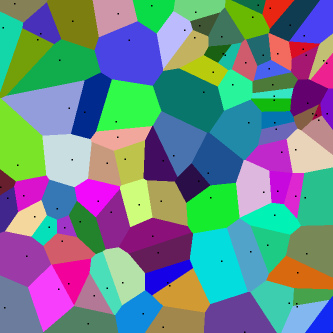
\includegraphics[width=0.15\textwidth]{assets/voronoi.png}
  \caption{Diagramme de Voronoï}
  \label{voronoi}
\end{wrapfigure}

Après la génération de nos terrains, nous prévoyons d'implémenter un système de biomes. Chaque biome, représentant une zone particulière du terrain, aura ses propres caractéristiques visuelles, avec des blocs dont les textures varieront selon le biome où ils se trouvent. Pour ce faire, il existe deux approches qui sont respectivement le Bruit Worley (ou Voronoï) et définir une carte avec des températures et une humidité.\par
La première approche a été créée par Steven Worley en 1996, et possède trois noms : le Bruit de Worley \cite{worley_noise}, le bruit de Voronoï et le bruit Cellulaire. Cette approche se base sur le diagramme de Voronoï \cite{voronoi_diagram}, qui est un découpage d'un plan sous forme de cellules.\par



Dans notre cas, cette méthode n'est pas forcément pertinente car elle est plus efficace sur un plan plutôt qu'en deux dimensions comme nous et les transitions entre les biomes seraient trop brutales.\par
\begin{wrapfigure}{r}{0.2\textwidth}
  \centering
  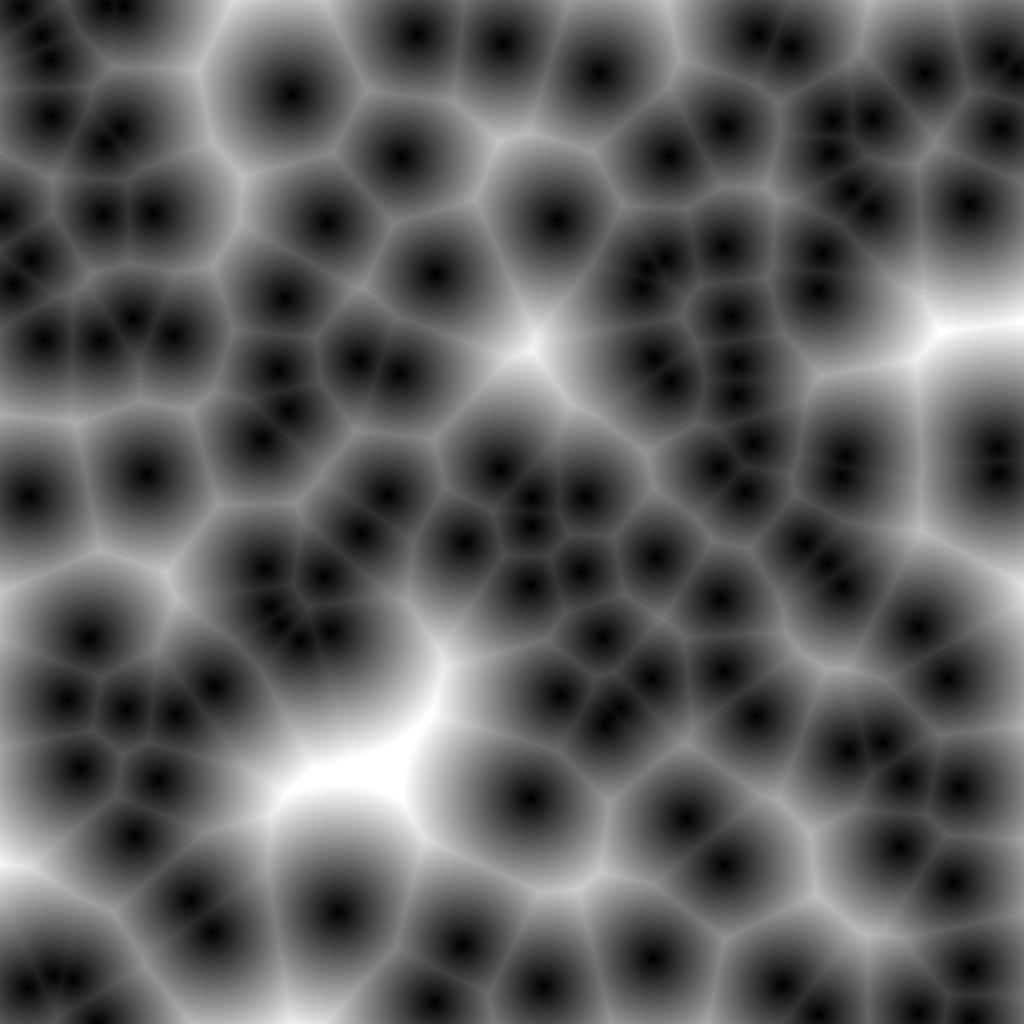
\includegraphics[width=0.15\textwidth]{assets/Worley.jpg}
  \caption{Bruit de Worley}
  \label{worley}
\end{wrapfigure}

La seconde approche serait donc optimale car on pourrait réutiliser les algorithmes pour la génération de terrains directement pour les biomes. En effet, le Bruit de Perlin, en plus de générer les terrains, peut également nous permettre de définir une humidité ainsi qu'une température pour chaque bloc, ce qui nous permettra d'avoir de meilleures transitions entre les biomes et permettre une expérience plus agréable au joueur. On s'orientera donc vers cette approche-là car elle correspond plus à nos besoins.
\par
Une fois notre terrain et nos biomes générés, afin de notre implémentation se rapproche le plus de Terraria, il faut générer des cavernes et des grottes souterraines. Il existe également deux approches différentes pour concevoir cela qui sont le Random Walk \cite{random_walk} (ou Marche Aléatoire) et une méthode qui utilise des automates cellulaires \cite{automate_cellulaire}.\par
\vspace{1cm}
\subsection{Génération de grottes et de cavernes}
\begin{wrapfigure}[7]{l}{0.2\textwidth}
  \centering
  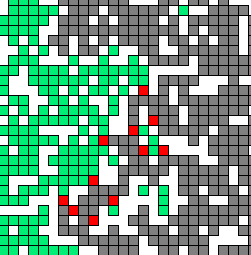
\includegraphics[width=0.18\textwidth]{assets/automate_cellulaire.png}
  \caption{Automate cellulaire}
  \label{automate_cellulaire}
  \vspace{0.5cm}
\end{wrapfigure}



La première méthode est un modèle mathématique qui permet de créer des donjons ainsi que des réseaux de tunnels. Nous nous focaliserons pas sur cette méthode car elle n'est pas utilisée par Terraria et que cela s'éloigne de la génération procédurale.\par 
La seconde méthode, utilisée par Terraria mais également par le jeu de la vie, consiste en une grille régulière de cellule, et une cellule évolue en fonction de ses voisines ce qui permet de générer des grottes réalistes.
\par
\vspace{2.5cm}
\subsection{Génération de minerais et ressources}
Maintenant que les grottes sont générées, il faudrait que le joueur puisse récolter des ressources. Nous n'irons pas aussi loin dans l'implémentation cependant nous générerons quand même des minerais. Il existe différentes méthodes qui permettent cela et qui sont la distribution par couches (ou Stratification \cite{stratification}) et le Bruit de Perlin appliqué au minerais. \par
La première méthode est utilisée par Minecraft en combinaison avec le Bruit de Perlin, la seconde se combine avec la génération de terrain et donc nous utiliserons cette méthode car c'est également celle utilisée par Terraria. Nous verrons plus en détail comment nous l'utiliserons pour notre implémentation à la section \ref{Implémentation}.
\vspace{1cm}
\subsection{Comparaison et choix des méthodes pour notre projet}

Comme nous avons pu le préciser lors des paragraphes précédents, la méthode de génération procédurale que nous utiliserons est le Bruit de Perlin car elle bien bien documentée et cela nous facilitera pour notre implémentation. De plus cette méthode nous sera également utile pour générer des biomes et des minerais, ce qui réduira de manière conséquente le travail réalisé. Enfin, pour générer nos grottes nous nous orienterons vers la méthode qui utilise les automates cellulaires car c'est la méthode utilisée par Terraria, cela nous paraît donc évident d'utiliser la même méthode. 
\newpage
\section{Méthodologie}

Nous avons vu ci-dessus les différents moyens d'appliquer la génération procédurale et les applications liées à ces moyens. Maintenant, nous devons définir une méthodologie afin de réaliser notre implémentation à partir des recherches effectuées.

\subsection{Les outils utilisés}

Afin de nous concentrer un maximum sur la recherche et l'application directe de la génération procédurale, nous avons choisi un langage que nous maîtrisons bien mais qui est bien documenté, Python. De plus, si nous voulons réaliser un jeu vidéo, nous ne pouvons pas le faire nativement et simplement, c'est pour cela que nous avons choisi le module Pygame, qui offre simplicité mais aussi une très bonne documentation, ce qui facilite l’appréhension de ce dernier.\par

\begin{figure}[!h]
  \centering
  \begin{subfigure}[b]{0.2\textwidth}
    \centering
    
\includegraphics[width=0.7\textwidth]{assets/python_logo.png}
    \caption{Logo Python}
  \end{subfigure}
  \hspace{0.6cm}
  \begin{subfigure}[b]{0.2\textwidth}
    \centering
    
\includegraphics[width=0.7\textwidth]{assets/pygame_logo.png}
    \caption{Logo Pygame}
  \end{subfigure}
  \caption{Logos des bibliothèques Python et Pygame}
  \label{fig:logos_python}
\end{figure}

Comme dit précédemment, nous connaissions déjà le langage python, nous n'avons donc pas eu beaucoup à apprendre. Cependant, le module Pygame était tout nouveau pour nous, nous nous sommes donc aidés de la documentation, de tutoriels sur YouTube mais aussi d'un livre \cite{prieur2019pygame}.\par
Puisque ce projet devait se réaliser en duo, il nous fallait à tout prix un outil pour travailler et collaborer. Dans un premier temps, pour la communication nous avons utilisé Discord, qui est très pratique car on peut échanger via des messages, des appels audios, vidéos mais cet outil offre également la possibilité de partager son écran directement en appel. Le second outil de collaboration utilisé est Git avec Github afin de partager le code. C'est actuellement sur le marché le meilleur outil de versioning et de collaboration. De plus, afin d'adopter une méthode agile et travailler sans se répeter, nous avons utilisés l'outil Jira. Il permet de créer des tickets qui correspondent à des tâches à effectués, puis de définir des périodes de Sprint, période où l'on effectue un ensemble de tickets.\cite{cochoy2011perlin}
\begin{figure}[!h]
  \centering
  \begin{subfigure}[b]{0.2\textwidth}
    \centering
    
\includegraphics[width=0.5\textwidth]{assets/discord.png}
    \caption{Logo Discord}
  \end{subfigure}
  \hspace{0.6cm}
  \begin{subfigure}[b]{0.2\textwidth}
    \centering
    
\includegraphics[width=0.6\textwidth]{assets/git.png}
    \caption{Logo Git}
  \end{subfigure}
  \hspace{0.6cm}
  \begin{subfigure}[b]{0.2\textwidth}
    \centering
    
\includegraphics[width=\textwidth]{assets/jira.png}
    \caption{Logo Jira}
  \end{subfigure}
  \caption{Logos des outils de communication et de collaboration}
  \label{fig:logos_collab}
\end{figure}
\vspace{1cm}
\subsection{Analyse du jeu}

Terraria est un jeu vidéo de type bac à sable, d'aventure et de construction développé par Re-Logic et publié en 2011 sur Steam. Aujourd'hui, il est disponible sur la plupart des plateformes et reste un incontournable dans son genre. Son principe est très simple, vous apparaissez dans un monde généré procéduralement, vous avez un inventaire avec des outils, et vous pouvez détruire des blocs et des arbres grâce à ces derniers. Votre inventaire sert également à poser des blocs et vous avez la possibilité de crafter\footnote{Crafter : assembler des ressources pour obtenir un objet} des objets (outils, blocs ou décoration).\par
La carte est une représentation verticale du monde, offrant une vue en deux dimensions. Ce dernier est composé d'une multitude de blocs qui forment des montagnes, des lacs, des forêts et des biomes en tout genre comme sur la figure \ref{surface}. On retrouve également toute une partie souterraine composée de blocs correspondant à des minerais collectables, de grottes et d'architectures variées, représentées sur la figure \ref{cavern}. Le joueur possède également la possibilité d'accéder à des souterrains en creusant sous ses pieds à l'aide d'une pioche.\par
L'objectif de notre implémentation est de réaliser l'aspect génération procédurale du jeu, ce qui représente la génération du terrain avec une notion d'altitude pour représenter des montagnes et des plaines. Nous implémenterons également une séparation du monde en plusieurs biomes pour diversifier la surface, et nous ajouterons un remplissage des sous-sols avec différents types de minerais, des blocs de pierre et des cavernes.
\vspace{1cm}

\begin{figure}[!h]
  \centering
  \begin{subfigure}[b]{0.4\textwidth}
    \centering
    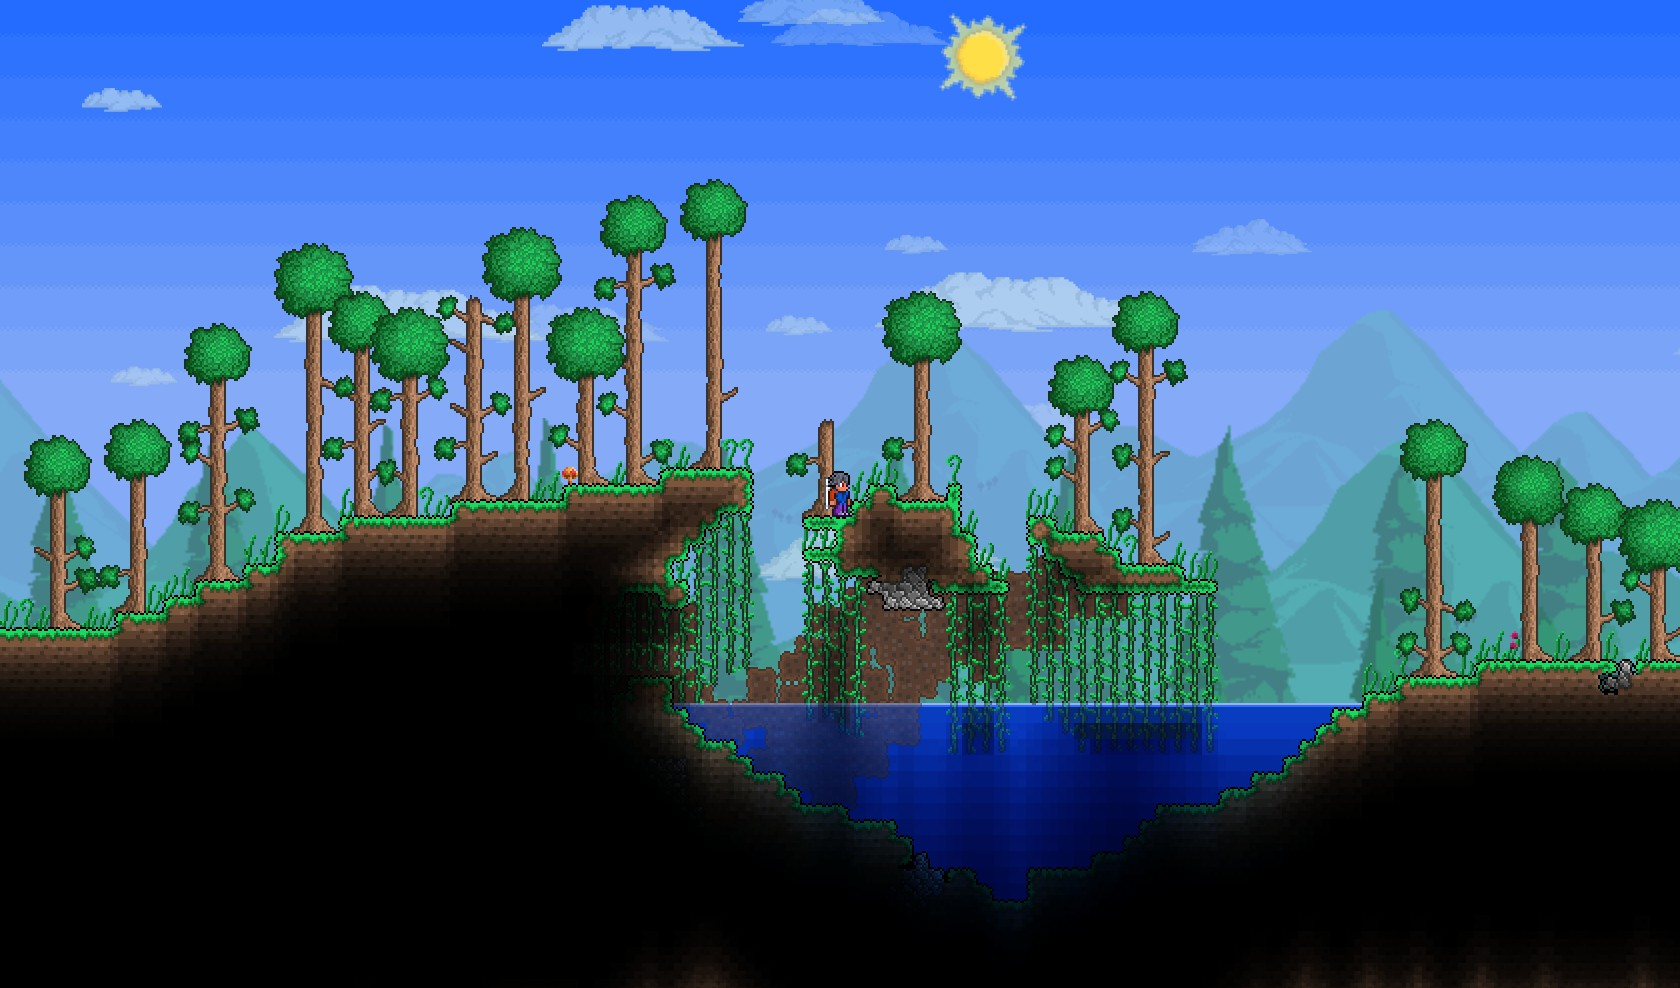
\includegraphics[height=95px]{assets/terraria_forest_biome.jpg}
    \caption{Surface du jeu}
    \label{surface}
  \end{subfigure}
  \hspace{1cm}
  \begin{subfigure}[b]{0.4\textwidth}
    \centering
    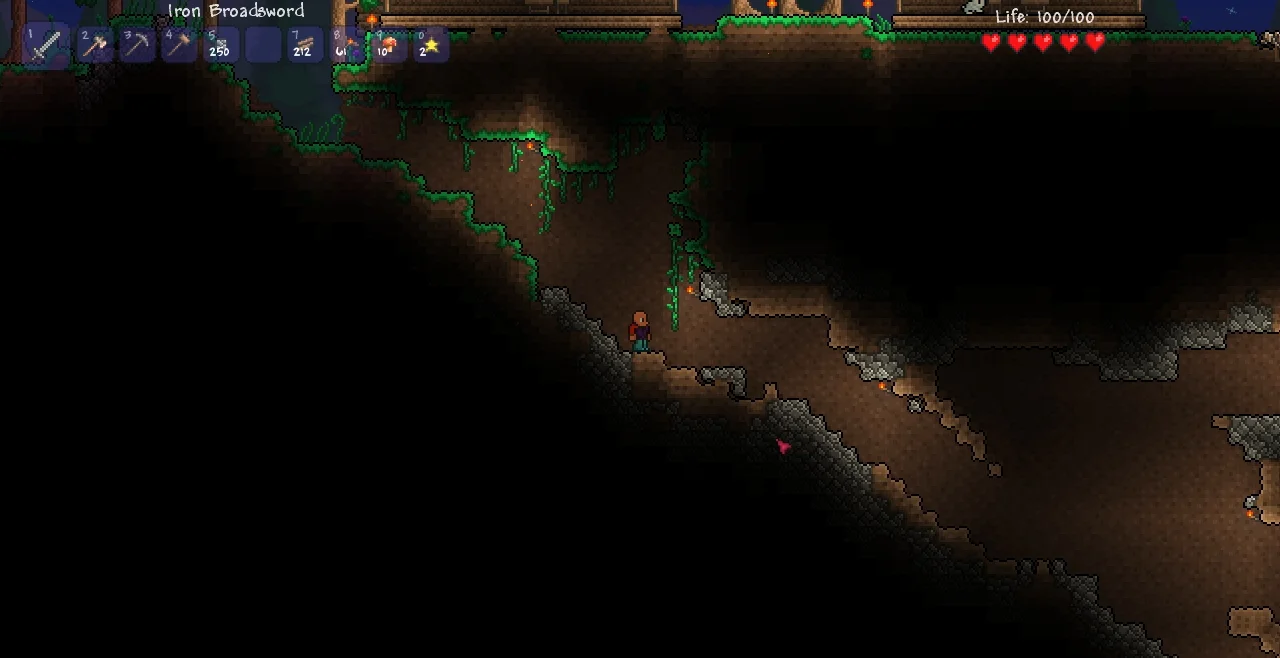
\includegraphics[height=95px]{assets/terraria_cavern.png}
    \caption{Sous-sol du jeu}
    \label{cavern}
  \end{subfigure}
  \caption{Exemple du jeu Terraria}
  \label{ImageJeu}
\end{figure}
\vspace{1cm}
\subsection{Organisation du code}

Pour avoir un code propre, et pour faciliter la compréhension entre nous, nous avons décidé au préalable d'une organisation et d'une structure de base. Le but était de créer un squelette de code qui nous permettrait de nous y retrouver facilement. Nous avons donc décidé de créer plusieurs fichiers, un pour chaque classe implémentée, chacun ayant une fonction précise. Nous avons pour cela créé un diagramme UML de classes que nous pouvons voir à la figure \ref{UML_class}.\par
Nous avons tout d'abord une classe Tile qui hérite de pygame.Sprite du module Pygame car elle propose des méthodes pour gérer les collisions de manière optimale avec les tuiles, et ses sous classes qui sont les différents types de blocs que l'on peut trouver dans le jeu. Ces blocs seront générés un à un procéduralement et seront destructibles, d'où l'utilité de les définir un à un.\par
Ensuite, nous avons la classe World qui va être la classe responsable de la génération du monde de manière procédurale. Elle va notamment avoir pour attribut une matrice de Tuiles car notre jeu est dans un espace à deux dimensions.\par
Puis, nous avons la classe Player qui va gérer le joueur, ses déplacements, ses interactions avec le monde et les blocs. Cette classe va hériter de classe pygame.Sprite.\par
Enfin, la classe Game qui va être la classe principale du jeu, elle va gérer la boucle principale du jeu, les événements, l'affichage et le rafraîchissement de l'écran.\par

\begin{figure}[!h]
  \centering
  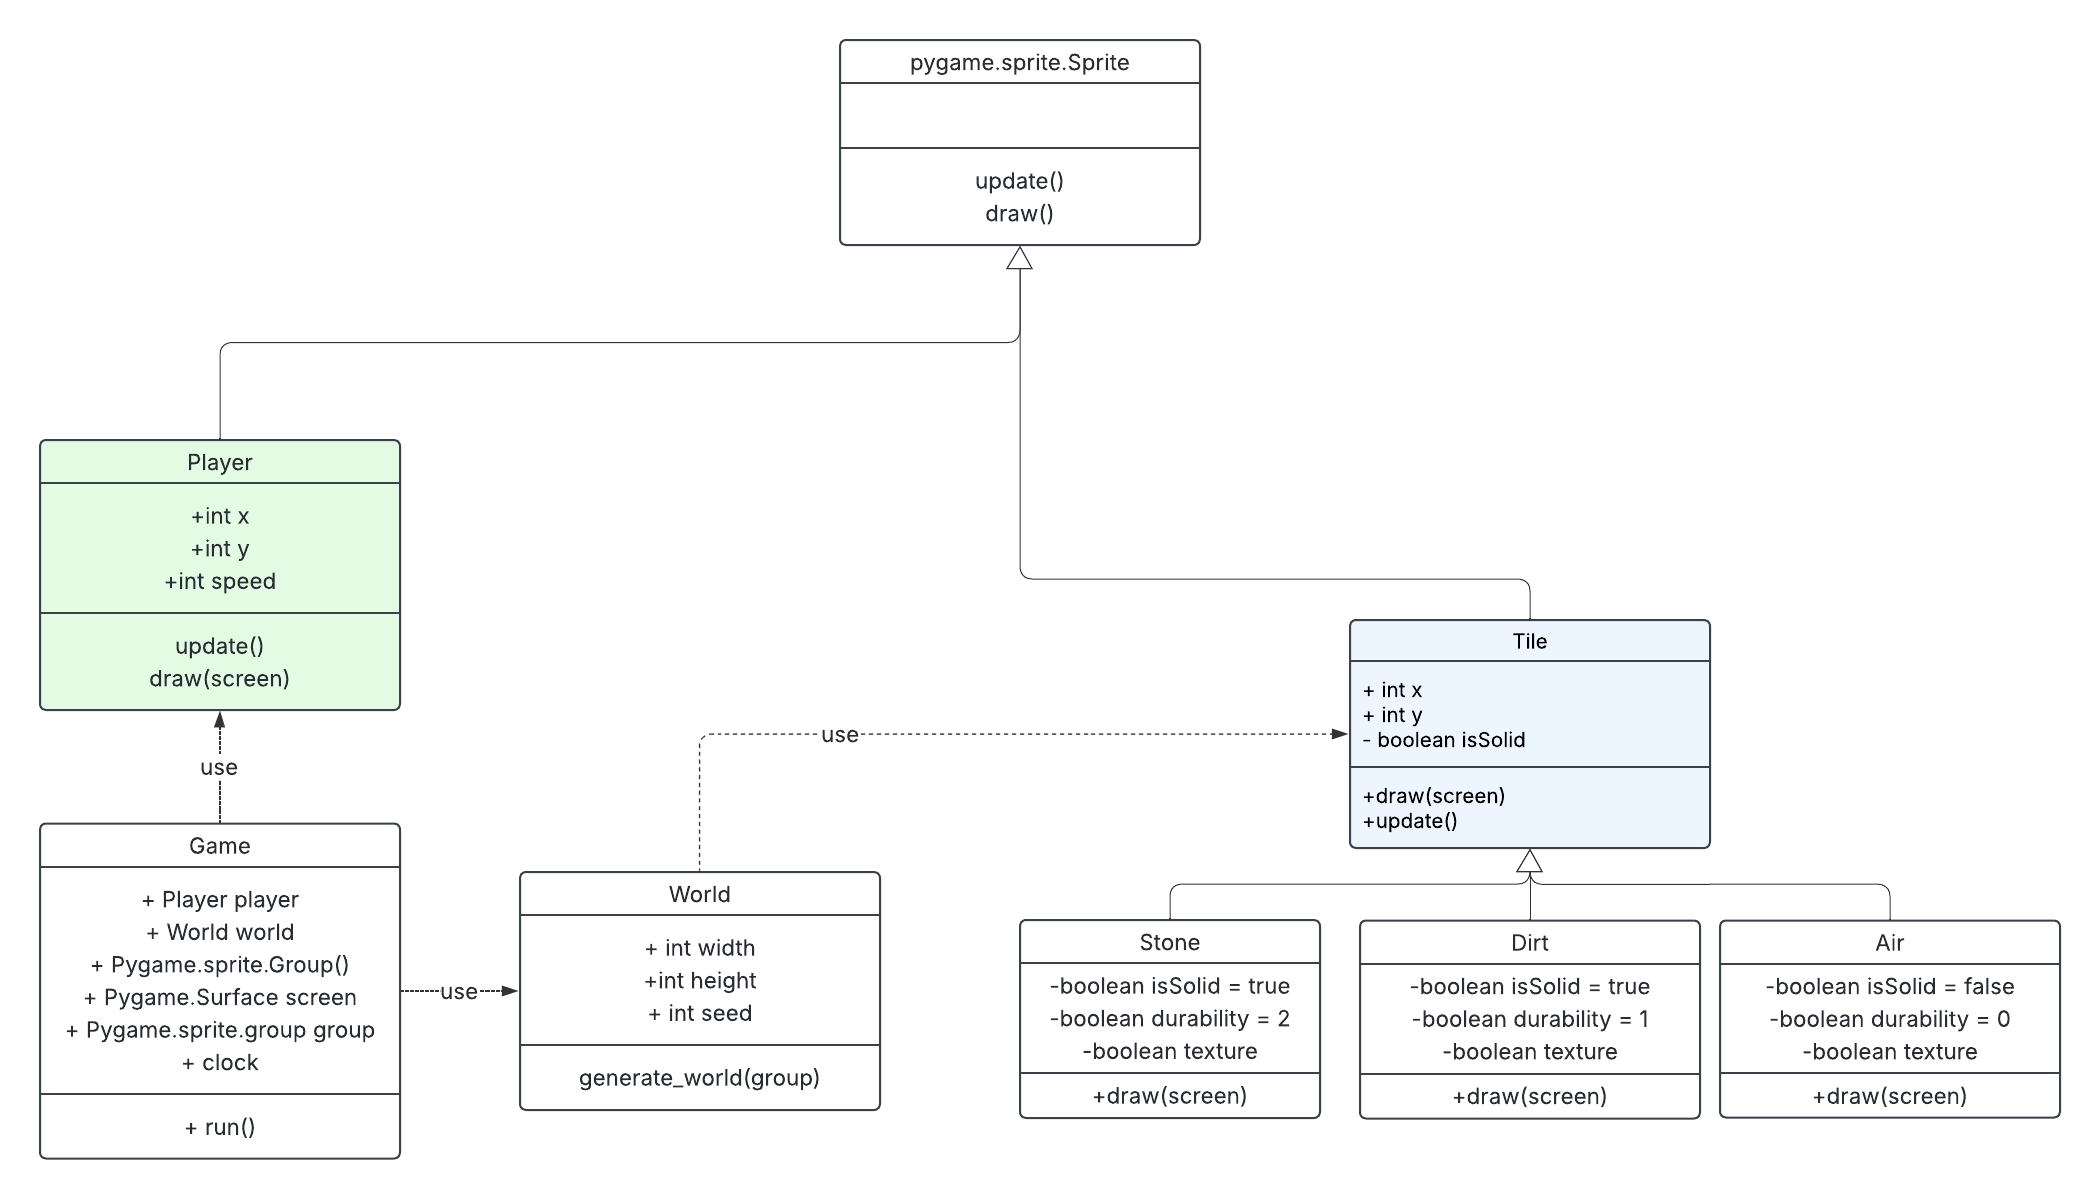
\includegraphics[width=\textwidth]{assets/UML_class.png}
  \caption{Diagramme de classe du Terraria-Like}
  \label{UML_class}
\end{figure}

Maintenant que nous avons définit comment nous allions aborder ce projet ambitieux, nous allons voir comment nous avons implémenté notre reproduction de Terraria.
\newpage
\section{Implémentation et Résultats}
\label{Implémentation}

Avant même de commencer à avoir un terrain qui se génère procéduralement, il a déjà fallut instaurer les bases de notre implémentation.

\subsection{Bases du jeu}

Tout d'abord, nous avons dû créer une fenêtre de jeu avec Pygame, puis définir la taille de la fenêtre. Ensuite, nous avons dû créer une boucle principale qui va gérer les événements du jeu, l'affichage et le rafraîchissement de l'écran avec trois méthodes qui sont respectivement \textbf{handling\_events}, \textbf{display} et \textbf{update}. Nous avons également dû définir un nombre de FPS (Images par secondes) afin d'avoir un affichage fluide et pas trop exigeant en ressources.\par
Une fois l'étape précédente réalisé, nous avons implémenté le joueur grâce à la classe Player. Ce dernier est défini par une boîte de collision, nommée \textbf{rect}, et une texture. Il peut se déplacer dans les quatre directions bien que le déplacement vers le bas corresponde à la gravité et le déplacement vers le haut à un saut. Lors-ce qu'il ce déplace, une animation est lui est appliquer en fonction de son mouvement et de sa direction. Pour ce faire nous nous sommes inspirés d'une playlist YouTube du Youtubeur Coding With Russ \cite{codingwithruss-playlist}. Cette dernière intègre des vidéos qui expliquent notamment les déplacements d'une entité dans Pygame.\par

\subsection{Génération procédurale du terrain}

La base de notre jeu est maintenant instaurée, avec un personnage qui peut se déplacer dans la fenêtre. Cependant, nous n'avons pas encore de décor, ni de monde. C'est ici que va intervenir la génération procédurale.\par
Nous nous sommes basés notamment sur un article parlant de la génération procédural écrit par Fabien Benoit-Koch \cite{benoitkoch} pour comprendre comment cela fonctionnait et comment y appliquer.
Puis, après quelques recherches nous nous sommes rendus compte qu'afin d'avoir un algorithme pas trop lourd à appliquer, nous allions nous baser sur le bruit de Perlin à une dimension.
Afin de bien comprendre comment nous nous y sommes pris dans un premier temps pour générer un terrain avec du relief, nous allons expliquer le fonctionnement du Bruit de Perlin à une dimension. Tout d'abord, nous avons définit un tableau de valeurs aléatoires entre -1 et 1 comme nous pouvons voir dans la figure \ref{tableau}.\par

\begin{figure}[!h]
  \centering
  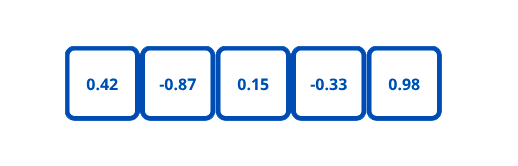
\includegraphics[width=0.6\textwidth]{assets/tableau.png}
  \caption{Exemple de tableau de valeurs aléatoires avec x égal à 5}
  \label{tableau}
\end{figure}

\newpage
Une fois que nous avons obtenu notre tableau de valeurs, nous allons le lisser 100 fois à l’aide du Bruit de Perlin. L’objectif est que, après avoir multiplié ces valeurs par une hauteur maximale (appelée valeur de y maximum), la différence entre deux valeurs voisines soit au maximum de 1. Cela permet d’obtenir une transition douce et progressive entre les valeurs, sans saut brusque comme nous pouvons voir sur le figure \ref{perlin1d}. Ce processus va donc nous permettre d'avoir un terrain avec du relief réaliste. En ce qui concerne les blocs placés et les textures, on choisit que la tuile la plus haute sur chaque colonne est un bloc d'herbe et les tuiles en dessous de la Terre. Par défaut, le reste des tuiles sont de l'air.\par % Peut être reformuler l'explication duu lissage
\begin{figure}[!h]
  \centering
  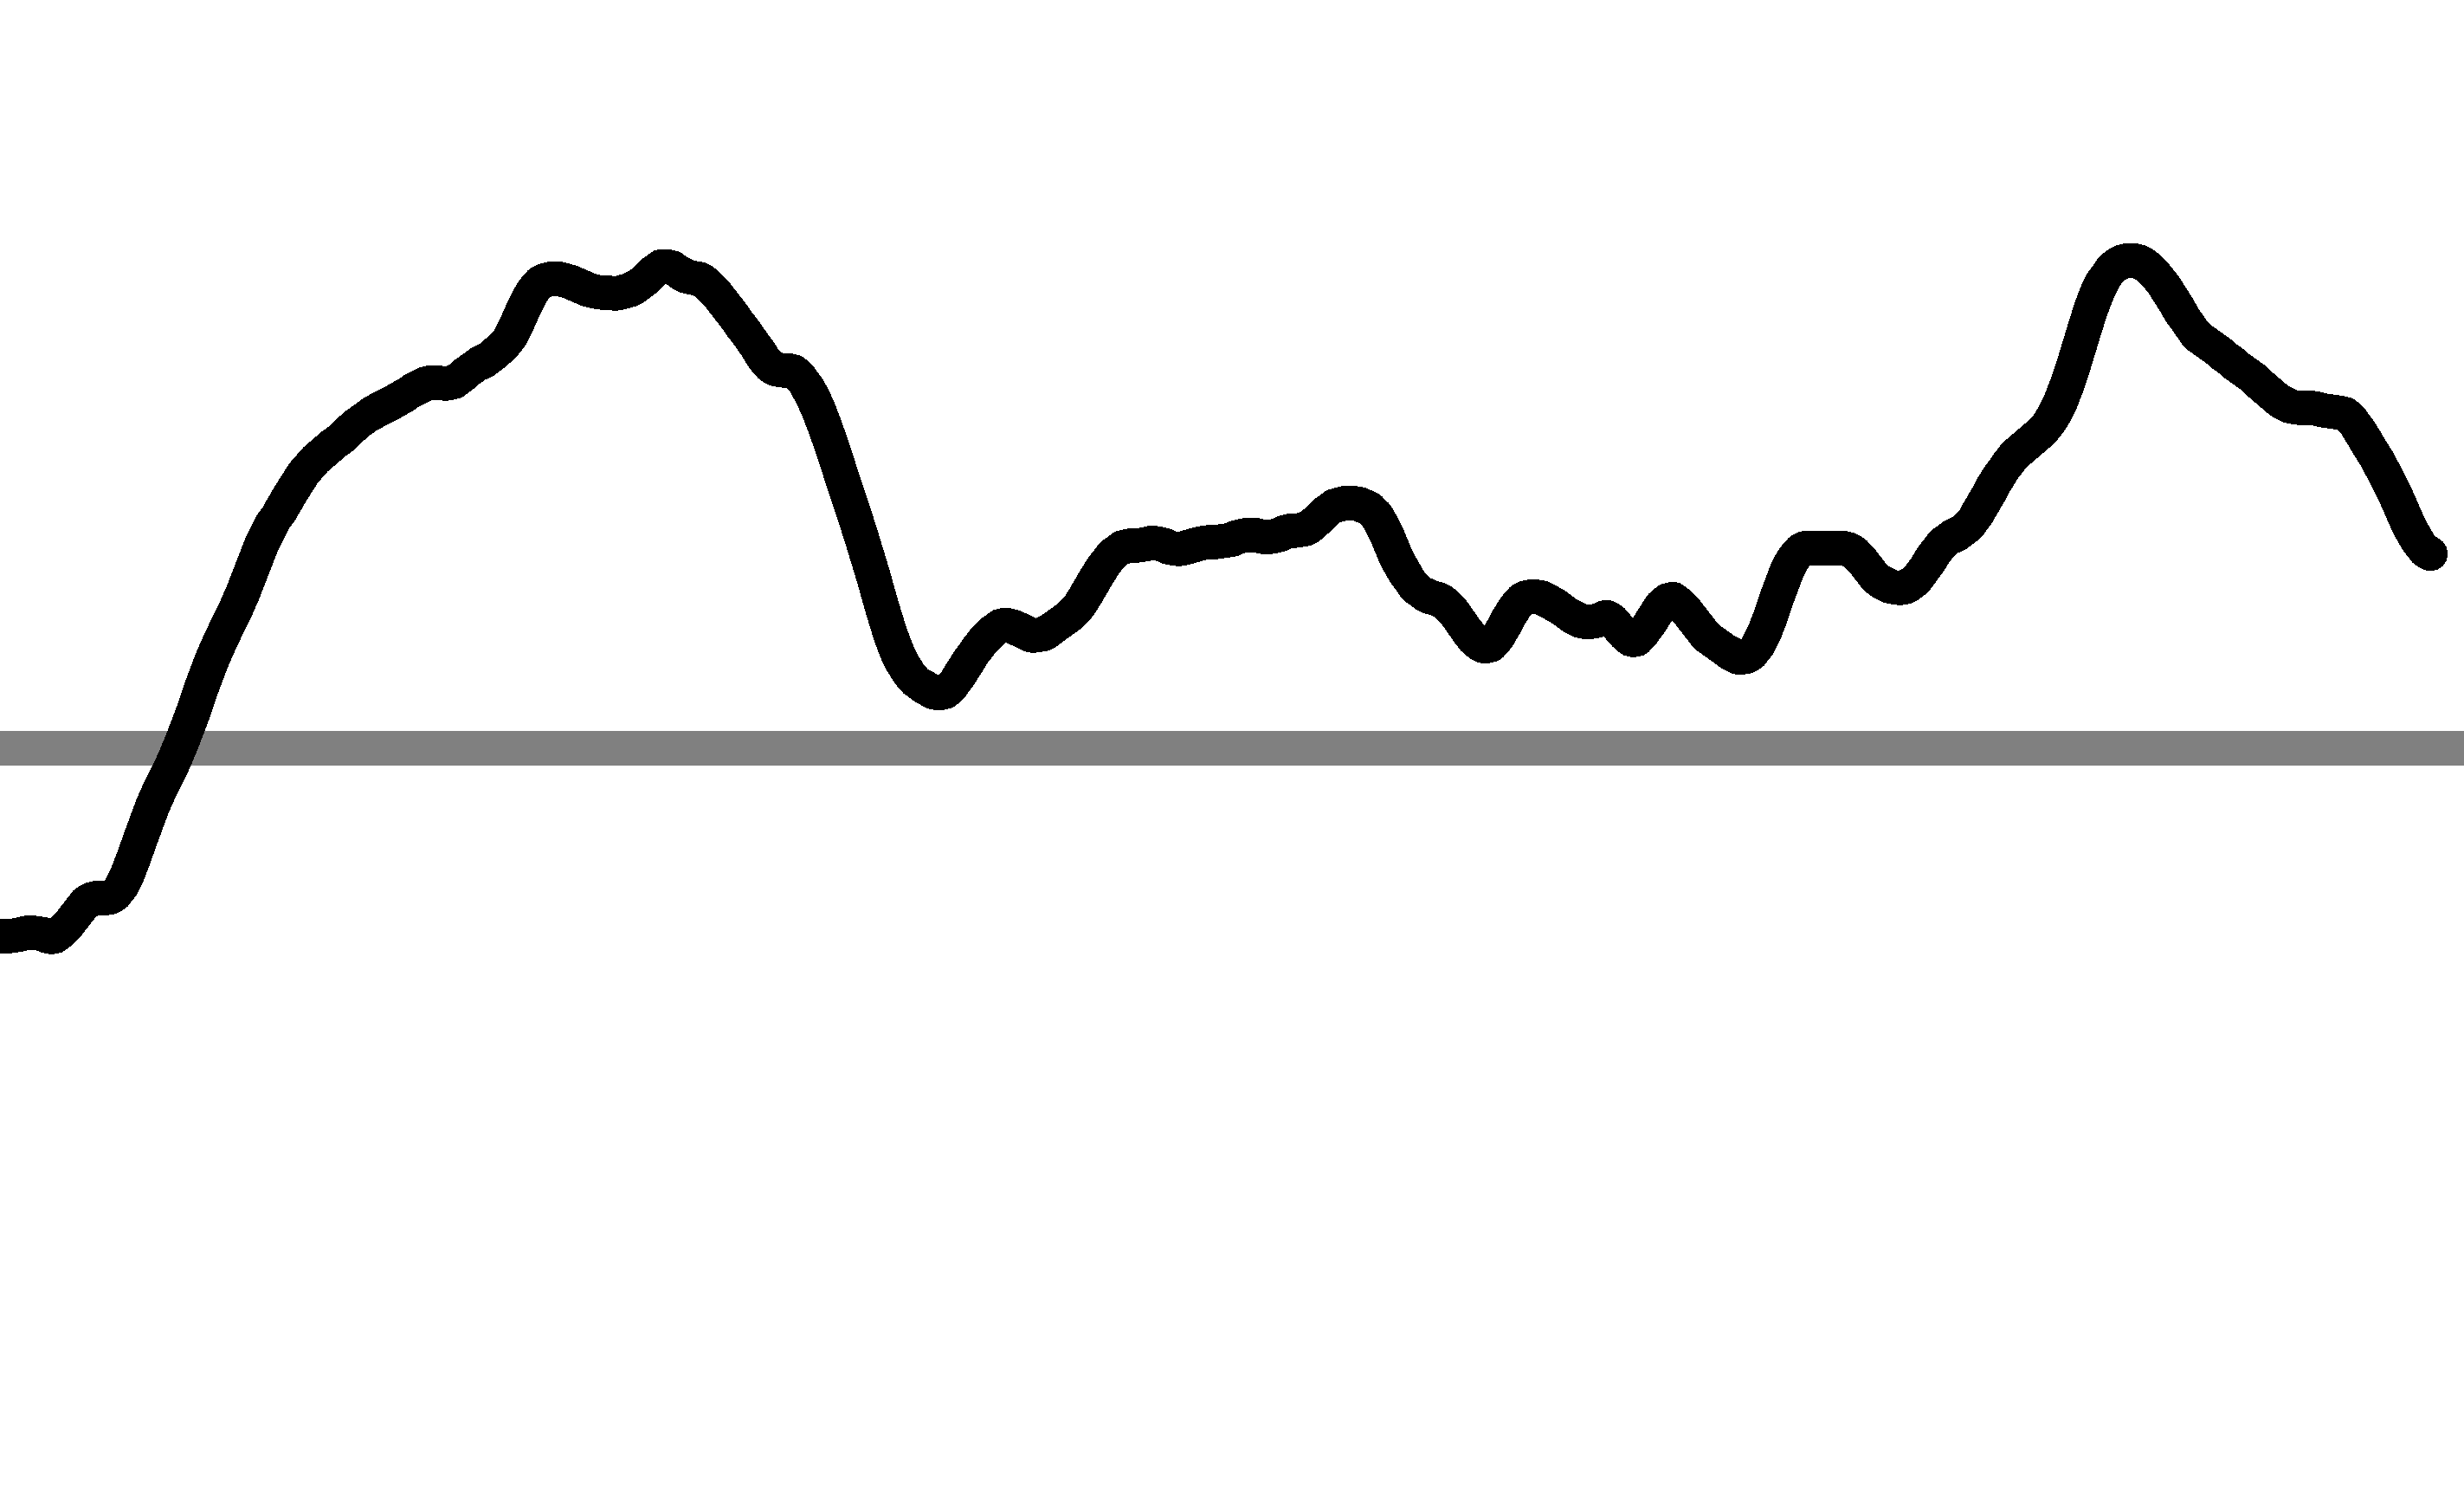
\includegraphics[width=0.5\textwidth]{assets/PerlinNoise1d.png}
  \caption{Bruit de Perlin à 1 dimension}
  \label{perlin1d}
\end{figure}

\subsection{Collisions}

Notre terrain est maintenant opérationnel et le joueur peut donc se déplacer dessus à une exception près, les collisions. En effet, bien que notre personnage puisse se déplacer, il peut passer à travers le terrain et les tuiles générées. Comme le joueur, les tuiles sont aussi définies par un \textbf{rect}. Nous avons donc utilisé la méthode \textbf{collide\_rect} de Pygame qui va détecter les collisions entre le joueur et les tuiles (sauf les tuiles de type air) grâce à leurs \textbf{rect}. Ensuite, il suffit juste de dire que le joueur ne peut pas se déplacer dans la direction de la collision et notre personnage pourra se mouvoir sur le terrain sans passer à travers. Pour réaliser cela, nous nous sommes servis des vidéos du Youtubeur \underline{Coding With Russ} \cite{codingwithruss-channel}. Pour éviter certains bugs de collision, le personnage est placé à un pixel du bloc avec lequel il allait entrer en collision plutôt que d'être collé à lui. Cette petite différence n'est pas visible à l'œil nu et nous évite de nombreux problèmes d'affichage. \par

\subsection{Fonctionnalités et optimisations}

Pour l'instant, notre personnage peut se déplacer sur le terrain mais peut sortir de la fenêtre du jeu. Or, le monde que nous générons fait quelques milliers de blocs de longueur et n'est pas affiché dans son entièreté. Il faudrait donc faire bouger la fenêtre en même temps que le joueur. Pour ce faire nous avons rajouté une caméra, représentée par un simple rectangle. Le personnage se situe toujours en son centre et tous les éléments de la carte sont affiché par rapport à la caméra.\par
\vspace{1cm}
Cette gestion de la caméra par un \textbf{rect} nous permet quelques fonctionnalités. Comme les éléments s'affichent par rapport à la caméra et non par rapport au joueur, alors on peut la déplacer volontairement pour offrir une vue spectateur. Le principe est simple, les touches ne font plus bouger le personnage mais la caméra, ce qui nous permet de nous déplacer rapidement quand l'on veut.\par 
L'utilisation des rectangles de Pygame nous permet également de faire quelques optimisations. Le jeu doit gérer une grande quantité de blocs et doit effectuer des calculs sur chacun d'entre eux, notamment en ce qui concerne les collisions. Cependant, seul le personnage peut interagir avec les blocs, alors il n'est pas nécessaire de faire des calculs sur ces derniers lorsqu'ils n'appartiennent pas à la zone d'affichage de la caméra. Pour aller encore un peu plus loin dans l'optimisation, nous n'affichons pas les blocs hors du champ de vision de la caméra et nous rendons le personnage immobile lorsque nous sommes en mode spectateur pour éviter qu'il tombe dans le vide.
\vspace{1cm}
\subsection{Génération procédurale des biomes}

Afin d'avoir une implémentation plus conforme au jeu de base, nous avons décidé de mettre en place un système de génération procédurale pour générer des biomes.
Un biome est une région qui présente différentes caractéristiques géographiques, notamment les végétaux, le climat ainsi que des espèces spécifiques. Deux paramètres très importants à prendre en compte dans un biome sont la température et l'humidité. En effet, là où la biome Jungle à la figure \ref{jungle} est chaud et sec, le biome Toundra à la figure \ref{toundra} est froid et sec. Pour réaliser cela, nous avons également utilisé le bruit de Perlin à une dimension pour chaque paramètre. Comme pour la génération procédurale de terrain, nous avons générés deux tableaux de valeurs aléatoires comprises entre -1 et 1, un pour la température et un pour l'humidité. Cependant, afin d'avoir moins de variations brusques entre chaque biome nous avons décidés de lisser 300 fois les valeurs générés entre 1 et -1 (contre 100 pour le terrain). 
On stockera ensuite dans un tableau, pour chaque valeur de x, le biome correspondant afin de nous faciliter la tâche quant au rendu visuel. Une fois notre tableau de biomes produit, nous avons, dans une fonction, définit des seuils qui permettent de définir un biome en fonction de la température et de l'humidité pour chaque valeur de x.\par
\vspace{1cm}

\begin{figure}[!h]
  \centering
  \begin{subfigure}[b]{0.4\textwidth}
    \centering
    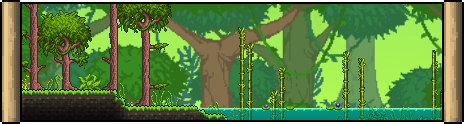
\includegraphics[width=0.9\textwidth]{assets/jungle.png}
    \caption{Biome Jungle}
    \label{jungle}
  \end{subfigure}
  \hspace{1cm}
  \begin{subfigure}[b]{0.4\textwidth}
    \centering
    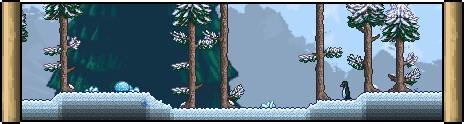
\includegraphics[width=0.9\textwidth]{assets/toundra.png}
    \caption{Biome Toundra}
    \label{toundra}
  \end{subfigure}
  \caption{Exemple de biomes du jeu Terraria}
  \label{biomes}
\end{figure}
\newpage
\subsection{Mécanique de destruction de blocs}

Pour permettre la destruction de blocs dans notre environnement, nous avons conçu une classe appelée \texttt{Selector}. Cette classe est chargée de positionner un indicateur visuel en fonction des coordonnées de la souris, facilitant ainsi l’interaction avec les blocs.

Le \texttt{Selector} a les mêmes dimensions qu’un bloc, ce qui garantit un alignement précis. Lorsqu’un utilisateur déplace la souris à l’écran, le \texttt{Selector} se déplace en conséquence, s’ajustant automatiquement pour se superposer au bloc ciblé dès que la souris entre en collision avec celui-ci. Cette approche simplifie la sélection des blocs et améliore l’expérience utilisateur en rendant l’interaction plus intuitive et réactive.\par
Une fois cette mécanique intégré, nous avons décidé de pouvoir détruire le bloc sélectionné par le \texttt{Selector}. Nous avons très simplement attendu qu'un clic gauche de souris soit effectué, si tel est le cas alors on détruit le bloc qui était sélectionné.\par
Dans le vrai jeu, cette mécanique possède une réelle plus-value car elle permet de creuser sous terre afin de récolter des minerais, pour ensuite fabriquer des outils, des armures, etc.


\vspace{1cm}
\subsection{Résultats}
Notre projet se présente sous la forme d’un jeu immersif dans lequel le joueur évolue au sein d’un monde ouvert, riche en reliefs et en biomes générés de manière procédurale.
\par
\vspace{0.3cm}
Nous pouvons notamment nous baser sur quelques points clés:\par
\vspace{0.3cm}
\begin{itemize}[label=\textbullet]
  \item 	\textbf{Déplacement du joueur} : Le joueur peut se déplacer librement à travers des environnements variés, chaque terrain étant généré procéduralement pour garantir une exploration unique à chaque partie (sauf si on utilise la même graine).
  \item \textbf{Gestion des collisions} : Pour renforcer l’aspect physique du jeu, nous avons intégré un système de détection des collisions, assurant que les interactions entre le joueur et les blocs restent cohérentes et naturelles.
  \item \textbf{Caméra dynamique} : La caméra suit automatiquement les mouvements du joueur, mais peut également être basculée en mode spectateur pour une exploration libre et aérienne du monde.
  \item \textbf{Modification du terrain} : Enfin, nous avons implémenté la possibilité de détruire des blocs, permettant ainsi au joueur de creuser.
\end{itemize}


\newpage
\vspace*{\stretch{1}}
\section{Conclusion et Perspectives}

L'objectif de ce projet était d'effectuer des recherches sur la génération procédurale et de coder une implémentation des différents algorithmes que nous avons pu étudier durant notre phase de recherches. Afin d'avoir une implémentation simple à comprendre et à présenter, et sur laquelle nous aurions eu du plaisir à développer, notre choix s'était porté sur Terraria. Le résultat final est cohérent, avec une génération procédurale des terrains et des biomes similaire au jeu d'origine. De plus, nous avons essayé de reproduire des textures qui se rapprochaient le plus de Terraria. Enfin, nous avons intégré des mécaniques de jeu comparables à celles du jeu de base, notamment les déplacements, le saut ou alors le cassage de blocs.\par
Nous avons donc réussi à répondre au cahier des charges en développant une implémentation de la génération procédurale. Nos biomes et nos reliefs se génèrent par rapport à une graine, c'est à dire que si la graine est la même alors le monde généré également. 

Cependant, nous n'avons pas implémenté la génération de grottes et de minerais par faute de temps. En effet, nous avons sûrement été très ambitieux quant à notre intégration. De plus, nous sommes conscients que notre optimisation pourrait être meilleure, notamment en gérant les collisions avec les blocs que seul le joueur pourrait toucher, mais également en faisant un système de chunks\footnote{Un chunk est une section de l’environnement du monde généré, s’étendant de la couche la plus basse à la plus haute du monde.}. Nous pouvons également rajouter le fait que nos algorithmes de génération procédurale ne nous permettent pas de faire de montagnes. C'est une amélioration que nous pourrons rajouter à l'avenir, afin d'avoir des hauteurs, notamment dans le biome montagnes.

Globalement, ce projet de recherche nous a été utile pour de nombreuses choses. Dans un premier temps, nous avons dû apprendre à effectuer des recherches efficaces pour mieux répondre à notre problématique. Cette étape du projet a été particulièrement intéressante, car elle nous a permis d’acquérir de nombreuses connaissances dans le domaine de la génération procédurale.\par
Dans un second temps, cela nous a appris à collaborer car c'est un des premiers projets de groupe que nous avons eu dans le cadre de notre licence. Cela nous aidera fortement pour l'avenir, notamment l'utilisation d'outils comme Jira ou Git.\par
Enfin, cette expérience nous a permis de renforcer nos compétences en programmation orientée objet et en Python. Nous avons structuré et organisé notre code de manière méthodique afin de faciliter la collaboration et d’assurer une maintenance efficace tout au long du projet. Cela nous a également appris l’importance des bonnes pratiques en développement, comme la modularité du code et l’utilisation de classes et d’héritage.
\vspace*{\stretch{1}}
\newpage
\vspace*{\stretch{1}}
\section{Remerciements}
Nous tenons à remercier notre responsable pour ce projet, Pierre-Cyrille Heam qui nous a accompagné mais également Julien Bernard pour nous avoir fourni un article très utile sur notre sujet.\par
Même si nous n’avons pas eu l’occasion de les rencontrer personnellement, nous souhaitons exprimer notre profonde gratitude envers l’ensemble des auteurs des articles que nous avons cités dans ce travail. Leur rigueur et leur partage de connaissances ont grandement enrichi notre réflexion et notre compréhension des sujets abordés.

Nous adressons également nos remerciements aux nombreux contributeurs de Wikipédia, dont l’effort collectif rend possible l’accès libre à une vaste source de savoir. Leurs contributions bénévoles ont été précieuses pour nos recherches et ont souvent servi de point de départ à notre travail.

Enfin, nous remercions les créateurs de contenu sur YouTube, dont les vidéos pédagogiques et explicatives ont su rendre certains concepts plus accessibles et concrets, facilitant ainsi notre apprentissage.
\vspace*{\stretch{1}}
\newpage
\section{Bibliographie et références}
\bibliographystyle{alpha}
\bibliography{bibliography}

\end{document}
